% Options for packages loaded elsewhere
\PassOptionsToPackage{unicode}{hyperref}
\PassOptionsToPackage{hyphens}{url}
%
\documentclass[
]{article}
\usepackage{lmodern}
\usepackage{amssymb,amsmath}
\usepackage{ifxetex,ifluatex}
\ifnum 0\ifxetex 1\fi\ifluatex 1\fi=0 % if pdftex
  \usepackage[T1]{fontenc}
  \usepackage[utf8]{inputenc}
  \usepackage{textcomp} % provide euro and other symbols
\else % if luatex or xetex
  \usepackage{unicode-math}
  \defaultfontfeatures{Scale=MatchLowercase}
  \defaultfontfeatures[\rmfamily]{Ligatures=TeX,Scale=1}
\fi
% Use upquote if available, for straight quotes in verbatim environments
\IfFileExists{upquote.sty}{\usepackage{upquote}}{}
\IfFileExists{microtype.sty}{% use microtype if available
  \usepackage[]{microtype}
  \UseMicrotypeSet[protrusion]{basicmath} % disable protrusion for tt fonts
}{}
\usepackage{xcolor}
\IfFileExists{xurl.sty}{\usepackage{xurl}}{} % add URL line breaks if available
\IfFileExists{bookmark.sty}{\usepackage{bookmark}}{\usepackage{hyperref}}
\hypersetup{
  pdftitle={Ecology Counts},
  pdfauthor={Odalys Barrientos, Brianna Cirillo, Veronia Marquez},
  hidelinks,
  pdfcreator={LaTeX via pandoc}}
\urlstyle{same} % disable monospaced font for URLs
\usepackage[margin=1in]{geometry}
\usepackage{graphicx,grffile}
\makeatletter
\def\maxwidth{\ifdim\Gin@nat@width>\linewidth\linewidth\else\Gin@nat@width\fi}
\def\maxheight{\ifdim\Gin@nat@height>\textheight\textheight\else\Gin@nat@height\fi}
\makeatother
% Scale images if necessary, so that they will not overflow the page
% margins by default, and it is still possible to overwrite the defaults
% using explicit options in \includegraphics[width, height, ...]{}
\setkeys{Gin}{width=\maxwidth,height=\maxheight,keepaspectratio}
% Set default figure placement to htbp
\makeatletter
\def\fps@figure{htbp}
\makeatother
\setlength{\emergencystretch}{3em} % prevent overfull lines
\providecommand{\tightlist}{%
  \setlength{\itemsep}{0pt}\setlength{\parskip}{0pt}}
\setcounter{secnumdepth}{-\maxdimen} % remove section numbering

\title{Ecology Counts}
\author{Odalys Barrientos, Brianna Cirillo, Veronia Marquez}
\date{}

\begin{document}
\maketitle

\hypertarget{statistical-methodology}{%
\section{Statistical Methodology}\label{statistical-methodology}}

In this analysis, contingency tables were used to asses how many journal
entries came from each of the independent variables used. A contingency
table, which can also be called a cross tabulation, is a table that
shows the frequency distribution of each of the variables. Data cleaning
was performed, thus removing any data where the independent variable
being looked at was not applicable. Therefore, we separated the data by
continent, country, region, state, and ecosystem. We looked at each of
these tables to determine if the number of journal entries in each
category, of these variables, were equal or close in frequency.

In order to better understand the distribution of the number of journal
entries in each category, pie charts and bar graphs were made. This gave
a visual representation of the distribution of journal entries in each
independent variable. Therefore allowing for a visual analysis based on
graphs and tables made.

To further analyze these categories, chi square tests were used to
determine whether or not the observed amount of journal entries for each
of the independent variables were equal. The Pearson's chi-squared test
is used to determine whether there is a statistically significant
difference between the expected frequencies and the observed frequencies
in one or more categories of a contingency table. An assumption of the
test is that observations are mutually exclusive and independent.
Therefore, data cleaning was done to ensure this condition was met. But
the data was not randomly sampled, which goes against one of the
assumptions. Thus, the p-values obtained do not have any relevance or
any real meaning in relation to the data.

Being that the data consists of predominantly categorical variables,
some additional data was added. Square mileage of continent, country,
region, and state were researched, in order to better estimate the
expected number of journal entries in each category.This allowed for chi
square tests to be run with expected frequencies, that match the square
mileage of each of the independent variables. This allowed for more
accurate expected frequencies of journal entries from each independent
variable. Data cleaning was done to remove rows that did not contain
applicable data for each independent variable. The assumption of random
sampling is still violated, therefore the p-values obtained could not be
used to draw conclusions.

\hypertarget{results}{%
\section{Results}\label{results}}

\hypertarget{a.-continent}{%
\subsection{a. Continent}\label{a.-continent}}

\hypertarget{b.-country}{%
\subsection{b. Country}\label{b.-country}}

\hypertarget{c.-region}{%
\subsection{c.~Region}\label{c.-region}}

\hypertarget{d.-state}{%
\subsection{d.~State}\label{d.-state}}

The state category noted if and how many of these published articles
completed their study in a particular state. This allowed us to see
which states were more or less popular for ecology work. The following
contingency table counts the number of times a state was represented in
the data set.

\begin{figure}
  \caption{Contingency Table}
    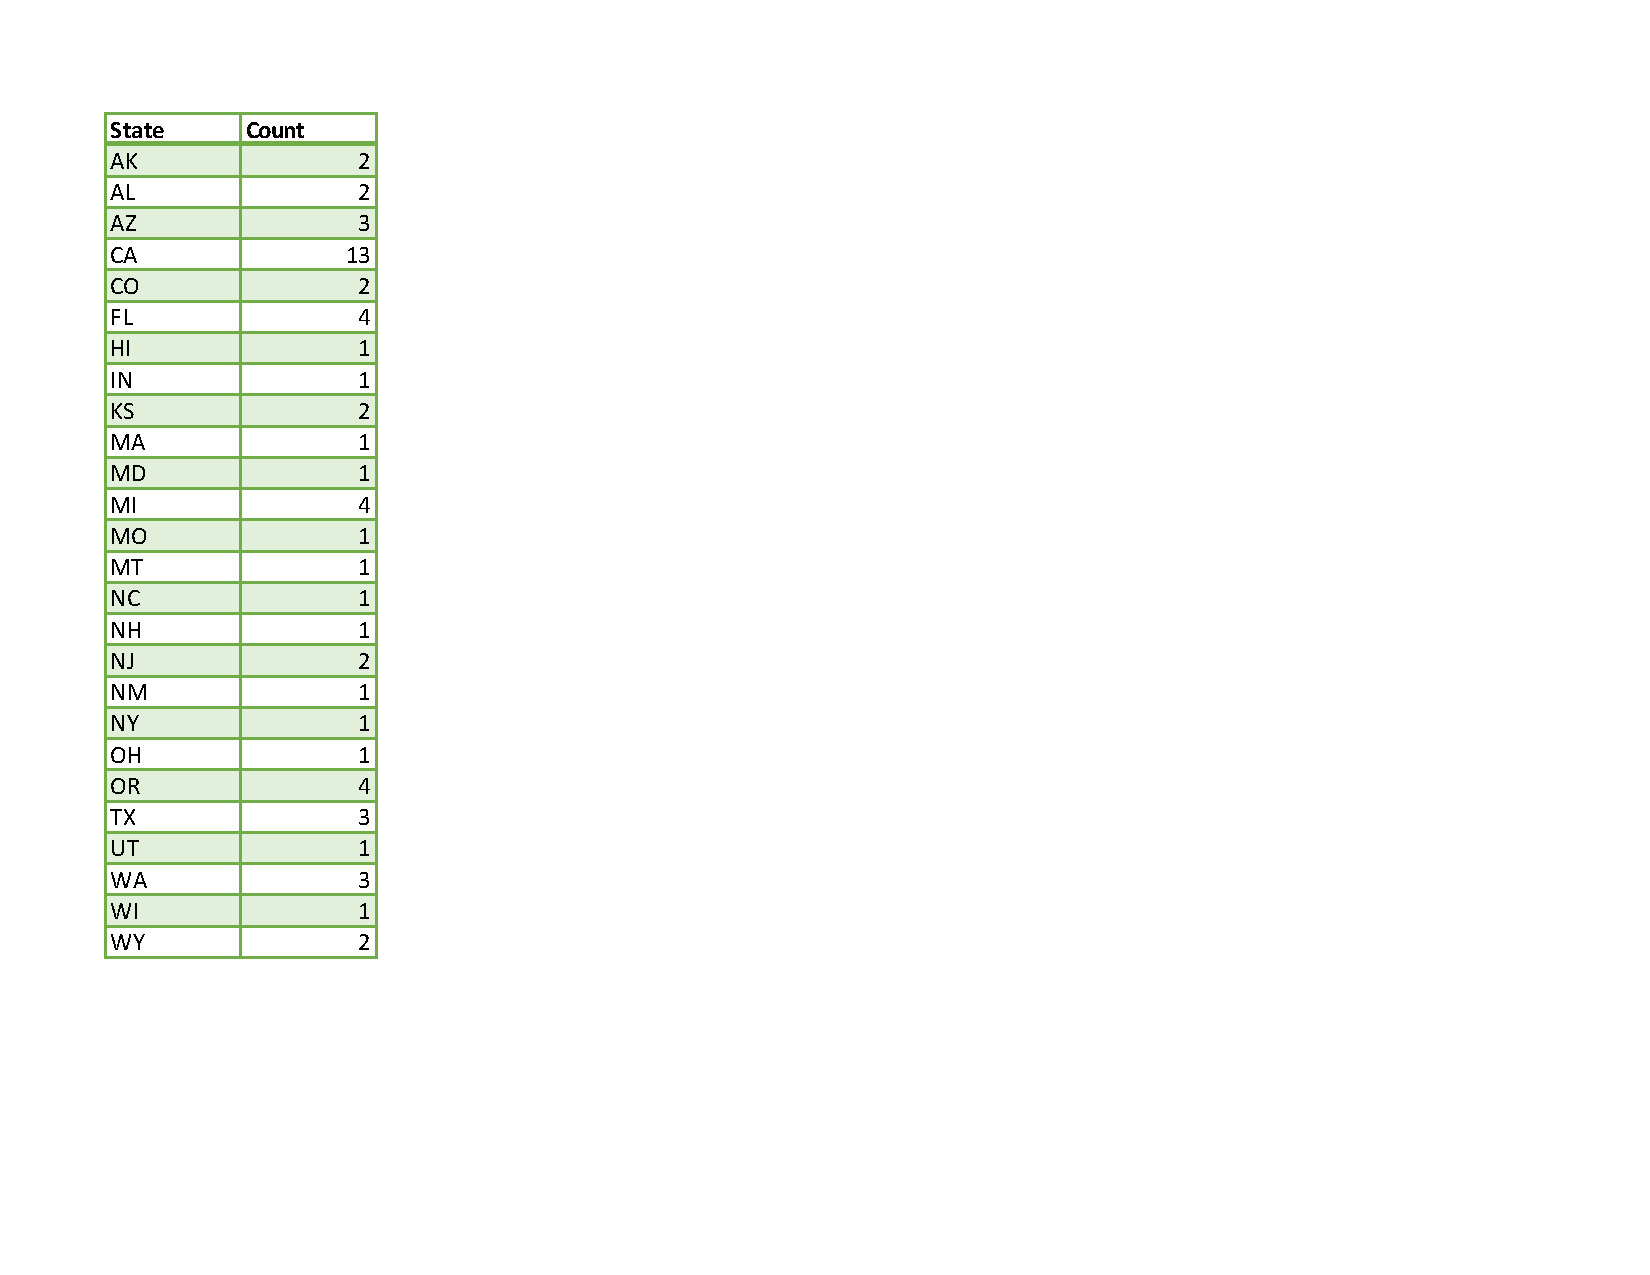
\includegraphics[width=13cm]{statetable.pdf}
\end{figure}

From the table above, one can tell that most of the journal entries are
published when the work was in California. The states that are not
included in the table were never represented in the data set.

If there is an assumption that the probability of each state being
represented in a journal entry is the same as each state's square
mileage then the larger states would have more published articles than
the smaller states. Below, is the Chi-Square test that test if this
statement is true.

insert fig

From the Pearson residuals one can note that California has the most
positive residual thus, the observed frequency exceeds the expected
frequency. For a visual presentation, figure \emph{3} helps explain this
idea. The map on the left is what the map is expected to look like based
off of how large and small each state is. The map on the right is what
the map looks like when using the counts from the data set.

\begin{figure}
  \caption{Expected Frequency based on Square Mileage}
    \includegraphics[width=13cm]{expected_map.pdf}
\end{figure}
\begin{figure}
  \caption{Observed Frequency}
    \includegraphics[width=13cm]{observed_map.pdf}
\end{figure}

California is a large state and the majority of the published articles
had work done in California. However, all the other states do not meet
the assumption. The gray states represent the sates that were never
counted in the data set. From the maps, one can conclude that the
probability of each state being represented in a journal entry is not
the same as the states square mileage. In other words, just because a
state is bigger does not mean there are more published articles from
that particular state.

\hypertarget{e.-ecosystem}{%
\subsection{e. Ecosystem}\label{e.-ecosystem}}

The ecosystem variable noted how many of the published articles used a
particular ecosystem. Ecosystems were broken down into 3 categories,
Marine, Terrestrial, and Freshwater. When looking at ecosystems, the
idea was to see if one ecosystem was counted more than a different
ecosystem. The following contingency table counts the number of times an
ecosystem was represented in the data set.

\emph{insert figure}

From the table above, one can tell that most of the published articles
have a terrestrial ecosystem.

If there is an assumption that the probability of each ecosystem being
represented in a journal entry is the same, then there should be the
same number of counts for each ecosystem. Below, is the Chi-Square test
that test if this statement is true.

\emph{insert figure}

From the Pearson residuals one can note that terrestrial has the most
positive residual thus, the observed frequency exceeds the expected
frequency. Additionally,freshwater has the most negative residual thus,
the observed frequency does not meet the expected frequency. For a
visual presentation, figure \emph{3} helps explain this idea. The pie
chart on the left shows what the pie chart should look like if every
ecosystem had an equal chance of being represented in a published
article. While the pie chart on the right is what the pie chart looks
like when using the counts from the data set.

\emph{insert figure}

If the ecosystems had a equal chance of being represented in these
published articles these pie charts would look similar. However this is
not the case and it is obvious that terrestrial takes up the majority of
the pie chart.

If there is an assumption that the probability of each ecosystem being
represented in a journal entry is the same as each ecosystem's square
mileage then the larger ecosystem's would have more published articles
than the smaller ecosystems. Below, is the Chi-Square test that test if
this statement is true.

\emph{insert figure}

Terrestrial has the most positive residual and marine has the most
negative residual. Figure \emph{3} shows what the expected counts should
look like and what the observed counts were.

\emph{insert figure}

These bar charts do not match up thus, we cannot conclude that the
probability of each ecosystem being represented in a journal entry is
the same as each ecosystem's square mileage.

\hypertarget{discussion}{%
\section{Discussion}\label{discussion}}

\end{document}
